% limen-guide-en.tex -- the guide to the limen package, set in limen itself.
% From the project root: make doc. Or here, if TeX can see limen: lualatex limen-guide-en.tex, three times.
\documentclass[10pt,a4paper]{article}
\usepackage[a4paper,left=58mm,right=17mm,top=30mm,bottom=29mm,headsep=8mm,footskip=11mm]{geometry}
\usepackage{fontspec}
% limen-guide-common.tex -- the layout shared by the guides. The guides load fontspec and their language first.
\setmainfont{Lora}[Path=../doc/fonts/,Extension=.ttf,UprightFont=*-Regular,BoldFont=*-Bold,
  ItalicFont=*-Italic,BoldItalicFont=*-BoldItalic,Ligatures=TeX]
\setsansfont{Inter}[Path=../doc/fonts/,Extension=.otf,UprightFont=*-Regular,BoldFont=*-SemiBold,
  ItalicFont=*-Italic,BoldItalicFont=*-Bold,Scale=0.9]
\linespread{1.1}
\usepackage{microtype}
\usepackage{fancyhdr,booktabs,tabularx,array,enumitem,caption,graphicx,fancyvrb,tikz}
\usepackage[hidelinks]{hyperref}
\usepackage[palette=ultramarine]{limen}
\limensetup{initialfont=fonts/Lora-Bold.ttf}
\graphicspath{{../gallery/}{gallery/}}
\definecolor{textc}{HTML}{1E1D22}
\definecolor{muted}{HTML}{5C5A63}
\definecolor{rulec}{HTML}{D6D3DE}
% chart colours, checked for separation under colour blindness and for contrast on the page
\definecolor{chartA}{HTML}{3D57C7}
\definecolor{chartB}{HTML}{B47A12}
\color{textc}
\hypersetup{colorlinks=true,linkcolor=limenink,urlcolor=limenink}
\makeatletter
\renewcommand\section{\@startsection{section}{1}{\z@}{-2.8ex plus -.6ex minus -.2ex}{1.2ex plus .2ex}%
  {\normalfont\large\bfseries\color{limenink}}}
\renewcommand\subsection{\@startsection{subsection}{2}{\z@}{-2ex plus -.4ex minus -.2ex}{.7ex plus .1ex}%
  {\normalfont\normalsize\bfseries\color{limenink}}}
\renewcommand\l@section{\@dottedtocline{1}{0pt}{1.6em}}
\renewcommand\numberline[1]{\hb@xt@\@tempdima{#1\hfil}}
\makeatother
\setcounter{secnumdepth}{1}
\setcounter{tocdepth}{1}
\pagestyle{fancy}\fancyhf{}\renewcommand\headrulewidth{0pt}
\fancyfoot[R]{\footnotesize\sffamily\color{muted}\thepage}
\setlist{leftmargin=1.2em,itemsep=2pt,topsep=3pt,parsep=0pt}
\setlist[itemize]{label={\color{limenaccent}\textbullet}}
\captionsetup{font={footnotesize,sf},labelfont=bf,labelsep=period,justification=raggedright,singlelinecheck=false,skip=5pt}
\setlength\parindent{0pt}\setlength\parskip{.55em plus .1em}
\emergencystretch=3em
\providecommand\curvesep{.}
% commands and options in the text
\newcommand\cs[1]{\texttt{\textbackslash #1}}
\newcommand\opt[1]{\texttt{#1}}
% tables
\newcolumntype{L}{>{\raggedright\arraybackslash\sffamily\footnotesize}X}
\newcolumntype{P}[1]{>{\raggedright\arraybackslash\sffamily\footnotesize}p{#1}}
\newcolumntype{T}[1]{>{\raggedright\arraybackslash\ttfamily\footnotesize}p{#1}}
\newcommand\thead[1]{\textbf{\sffamily\footnotesize #1}}
\newcommand\fig[3][1]{\par\medskip\noindent\begin{minipage}{\linewidth}\includegraphics[width=#1\linewidth]{#2}\captionof{figure}{#3}\end{minipage}\par\medskip}
\DefineVerbatimEnvironment{code}{Verbatim}{fontsize=\small,formatcom=\color{limenink},xleftmargin=.6em,samepage=true}
% the curve of the story, computed by the package itself; #1 lists thresholds as shares of the document
\newcommand\curvepts[1]{\directlua{
  local Art = require("limen-art")
  local ths = {}
  for v in string.gmatch("#1", "[0-9.]+") do table.insert(ths, { i = tonumber(v) * 100 + 1, y = 1 }) end
  local S = Art.make_story(1, 1, Art.defaults(), { pages = 100, ths = ths })
  local t = {}
  for k = 0, 200 do table.insert(t, "(" .. k / 200 .. "," .. S.curve(k / 200, 0.04, 0.07) .. ")") end
  tex.sprint(table.concat(t, " -- "))}}
% #1 x label, #2 y label, #3 legend of one threshold, #4 legend of three, #5 caption
\newcommand\curvefig[5]{\par\medskip\noindent\begin{minipage}{\linewidth}\centering
  \begin{tikzpicture}[x=.88\linewidth,y=34mm,font=\sffamily\footnotesize]
    \foreach \v/\t in {0/0,.5/0\curvesep 5,1/1} {\draw[rulec,line width=.3pt] (0,\v) -- (1,\v); \node[anchor=east,text=muted] at (0,\v) {\t};}
    \foreach \v/\t in {0/0,.25/0\curvesep 25,.5/0\curvesep 5,.75/0\curvesep 75,1/1} {\draw[rulec,line width=.3pt] (\v,0) -- (\v,-.03); \node[anchor=north,text=muted] at (\v,-.03) {\t};}
    \edef\limentmp{\noexpand\draw[chartB,line width=1.3pt,line join=round] \curvepts{0.18,0.5,0.75};}\limentmp
    \edef\limentmp{\noexpand\draw[chartA,line width=1.3pt,line join=round] \curvepts{0.25};}\limentmp
    \node[anchor=north,text=muted] at (.5,-.14) {#1};
    \node[anchor=south,rotate=90,text=muted] at (-.07,.5) {#2};
    \draw[chartA,line width=1.3pt] (0,1.13) -- (.05,1.13); \node[anchor=west] at (.05,1.13) {#3};
    \draw[chartB,line width=1.3pt] (.42,1.13) -- (.47,1.13); \node[anchor=west] at (.47,1.13) {#4};
  \end{tikzpicture}
  \captionof{figure}{#5}\end{minipage}\par\medskip}

\hypersetup{pdftitle={limen: the guide},pdflang={en}}
\fancyhead[R]{\footnotesize\sffamily\color{muted}limen: the guide}

\begin{document}
\limencover{limen}{Page margins where light has to earn its colour}{Guide to version 0.2\\November 2026}

\limeninitial{L}imen (Latin for threshold) is a LuaLaTeX package that draws a night field, fine lines of equal phase and a beam in the margin. At every heading the beam closes into a white star; between headings it opens into a spectrum. Everything is computed in Lua while the page ships and written straight into the PDF: no images, no external files.

The point is the story, more than the picture. On the first pages the beam is thin and almost white, the field is dark and the lines are only beginning to show. At the threshold the growth begins, and at the end of the document the full spectrum leaves through the edge of the sheet. A document gets a development you can see just by leafing through it. This guide shows how it works, because it is set in the package itself.

\fig{story.png}{The margins of an eight-page document in a row: below the threshold, the threshold, the rise, the end.}

\begingroup\small\setlength\parskip{0pt}\tableofcontents\endgroup

\section{When to use it}

The style is bright and strongly changes how a document comes across. It does not suit everything. Here is how to decide.

\medskip
\noindent\begin{tabularx}{\linewidth}{@{}P{42mm}L@{}}
\toprule
\thead{Good for} & \thead{Why}\\\midrule
Writing about light, lasers, optics, spectroscopy, radiation & The image belongs to the subject\\
Analyses, lab reports, explainers, handouts & People read them by choice, and the design helps the document stand out\\
Documents with a turn: ``it seemed like this, and in fact it is that'' & The threshold stands on the turn, so the picture serves the argument\\
Reading on screen, 3 to 40 pages & The story needs room, and a dark margin needs no printer\\
Talks and seminars & Usually 10--30 slides, and the rise shows well on a screen\\
\bottomrule
\end{tabularx}

\medskip
\noindent\begin{tabularx}{\linewidth}{@{}P{42mm}L@{}}
\toprule
\thead{Better avoided} & \thead{What instead}\\\midrule
Journal submissions, contracts, official forms & The format is prescribed. Use the publisher's template\\
Office printing in the dark mode & \opt{mode=paper}: a light field uses far less ink\\
One or two pages & The story has no room. Use \opt{story=flat}\\
Wide tables and figures on every page & The column takes about 5~cm. Widen those pages, see section~\ref{recipes}, or do without the package\\
Long books & One rise over hundreds of pages goes unnoticed. Use \opt{story=chapter}\\
Topics unrelated to light & The image becomes arbitrary, and readers will look for a meaning in it\\
Documents seen from one open page & The first pages are quiet on purpose. Move the threshold towards the start\\
The rainbow distracts, but the beam matters & \opt{beam=mono}: one colour, like a real laser\\
\bottomrule
\end{tabularx}

\section{Start}

You need LuaLaTeX and LaTeX from October 2020 or later. The 2023 and 2026 releases have been tested, see section~\ref{checked}. The package does not work with pdfLaTeX or XeLaTeX, because all of the art is computed in Lua.

To install, put \opt{limen.sty}, \opt{limen.lua}, \opt{limen-art.lua}, \opt{limen-pdf.lua} and \opt{limen-palettes.lua} next to your document. To make the package visible to every document, run \opt{make install}.

\begin{code}
\documentclass[10pt,a4paper]{article}
\usepackage[left=58mm,right=17mm,top=30mm,bottom=29mm]{geometry}
\usepackage[palette=ultramarine]{limen}
\begin{document}
\section{Below the threshold}
...
\end{document}
\end{code}

Run LuaLaTeX twice, as for a table of contents, because the story needs the length of the document. \opt{latexmk -lualatex} takes the right number of runs by itself. If the length has changed, the package says in the log that another run is needed.

Working with the package usually comes down to three steps.
\begin{enumerate}[leftmargin=1.5em]
\item \textbf{Free the margin.} The art takes the whole left margin. On A4, 58~mm works well. If the column gets narrower than 2.5~cm, the package warns you.
\item \textbf{Choose a palette.} Usually by laser or by subject, see section~\ref{palettes}.
\item \textbf{Place the threshold.} \cs{limenthreshold} on the turn of the argument. If there is no turn, the threshold stays at 25~\% of the document.
\end{enumerate}
The package takes care of headings, the rise and the end. The text and its page breaks do not depend on the art, which the tests check.

\section{The story}
\limenthreshold

The threshold of this guide stands right at the heading ``The story''. Look at the left margin: up to here the beam was white, and here colour begins.

The curve follows a laser's output against its pump power: almost nothing below the threshold, then a nearly straight rise. With several thresholds it climbs in steps: each one starts a rise that settles before the next.

\curvefig{Share of the document}{How far the spectrum opens}{One threshold, 0.25}{Three thresholds: 0.18, 0.5 and 0.75}{How the spectrum opens through a document. The curves come from the same code that draws the margins.}

The width of the spectrum, the colour of the field, the brightness of lines and caustics and the size of stars all follow this curve. The rise is continuous, also within a page, so the threshold shows as an event on one particular sheet and not as a jump between sheets.

\begin{itemize}
\item \cs{limenthreshold} places the threshold at this point in the text. The star here is larger than the others. Several of these make steps.
\item \opt{threshold=0.1} gives the threshold as a share of the document, when there is no turn to mark.
\item \opt{story=flat,level=0.7} turns the rise off and holds one stage, for short texts.
\item \opt{story=chapter} starts the story again in every chapter. In classes without chapters, \cs{limenrestart} does the same.
\item \cs{limenlevel\{0.9\}} sets the stage by hand from the page where it stands. An empty \cs{limenlevel\{\}} returns to the normal course.
\item \cs{limenend} ends the story earlier, before appendices for example. Without it the end is on the last page.
\end{itemize}

A star always means a heading or a mark in the text. On a long stretch without headings the beam only narrows; if you want a star there, \cs{limenstar} places it.

If the closing page has a lot of room left, the night field spreads below the text, and the beam passes a large caustic and leaves through the right edge as a fan. The page number turns white by itself there, with any page style. With less room the fan is small and leaves through the left margin.

\section{Options}

Options go in when the package is loaded, or in the preamble through \cs{limensetup\{...\}}.

\medskip
\noindent\begin{tabularx}{\linewidth}{@{}T{26mm}P{33mm}L@{}}
\toprule
\thead{Option} & \thead{Values} & \thead{Effect}\\\midrule
palette & see section~\ref{palettes} & Colours of the field, lines and headings\\
mode & night, paper & Dark field for the screen, light one for a printer\\
story & threshold, flat, chapter & One rise, one fixed stage, or a rise in every chapter\\
threshold & 0--0.9, default 0.25 & Where the threshold is, without \cs{limenthreshold}\\
level & 0--1, default 0.75 & The stage of \opt{story=flat}\\
beam & spectrum, mono & A rainbow, or one colour like a real laser\\
wavelength & nm & The wavelength with \opt{beam=mono}. By default the palette's own\\
caustic & ellipse, cardioid, nephroid, rings, speckle, mix & Kind of caustics\\
caustics & 0, 1, 2 & At most this many caustics on a page\\
density & 0.2--3, default 1 & How many lines of equal phase\\
lines & true, false & Lines of equal phase\\
headings & true, false & Stars at headings\\
finale & true, false & The closing fan\\
headrule & true, false & The rule above the text\\
column & cm & Width of the coloured column. By default it reaches the text\\
seed & number & A different picture with the same story\\
paper & HTML colour & Paper colour if it is not white, together with \cs{pagecolor}\\
initialfont & auto, a file & Font of the initials. By default the document's bold face\\
color & rgb, cmyk & Colour model of the art, see section~\ref{paper}\\
bleed & mm & Bleed on each side of the sheet, see section~\ref{paper}\\
sameart & true, false & The same picture on every page, for animations\\
draft & & No art: fast builds while editing the text\\
\bottomrule
\end{tabularx}

\section{Commands}

\medskip
\noindent\begin{tabularx}{\linewidth}{@{}T{52mm}L@{}}
\toprule
\thead{Command} & \thead{Effect}\\\midrule
\textbackslash limenthreshold & The threshold is here\\
\textbackslash limenstar & A star on the beam beside this line\\
\textbackslash limencaustic[kind=rings,size=1.3] & A caustic beside this line: its kind and radius in centimetres\\
\textbackslash limenrestart & A new story, with \opt{story=chapter}\\
\textbackslash limenlevel\{0.9\} & The stage by hand, from this page on\\
\textbackslash limenpause & No art on this page\\
\textbackslash limenoff, \textbackslash limenon & Art off and on again\\
\textbackslash limenend & The story ends here and not on the last page\\
\textbackslash limeninitial[3]\{T\}his & An initial three lines tall. The word still copies and searches as a whole\\
\textbackslash limenrule[0.5\textbackslash linewidth] & A divider: a thin spindle of spectrum\\
\textbackslash limenspark[0.8em] & A glint the size of a letter\\
\textbackslash limenspectrum[4cm] & A strip of spectrum, 400 to 700~nm\\
\textbackslash limencover[style=dark]\{\}\{\}\{\} & A cover: title, subtitle, details\\
\textbackslash limendefinepalette\{name\}\{...\} & Your own palette, in the preamble\\
\textbackslash limensetup\{...\} & Change options, in the preamble\\
\bottomrule
\end{tabularx}

\medskip
The colours \opt{limenink} and \opt{limenaccent} are there for your headings and bullets, so that the text matches the margin.

\section{Palettes, beam and caustics}\label{palettes}

\fig{palettes.png}{From left to right: ultramarine, peacock, ruby, emerald, infrared, graphite. The last page of each.}

\begin{itemize}
\item \opt{ultramarine}. The main one: blue night and gold lines. It suits almost anything, and the rainbow shows best on it.
\item \opt{peacock}. Teal and emerald. Softer, but the colour of the field competes a little with the beam.
\item \opt{ruby}. The ruby laser, 694~nm. Warm and dramatic.
\item \opt{emerald}. The second harmonic of Nd:YAG, 532~nm.
\item \opt{infrared}. Nd:YAG itself, 1064~nm, in the colours of a thermal camera.
\item \opt{graphite}. No colour in the field: only the beam has any. The most restrained one.
\end{itemize}

Your own palette goes in the preamble. No key is required; missing ones come from \opt{ultramarine}.
\begin{code}
\limendefinepalette{dusk}{deep=1B1033, flow=5A2A7A, flow2=A83E6A,
  line=FFD9A0, caustic=FFC48A, ink=5A2A7A, accent=C9773A}
\limensetup{palette=dusk}
\end{code}
Here \opt{deep} is the night, \opt{flow} and \opt{flow2} the slow currents on it, \opt{line} the lines, \opt{caustic} the caustics, \opt{ink} and \opt{accent} the colours for the text. Keep the field dark: the beam only glows on a dark one.

\textbf{One colour.} With \opt{beam=mono} there is no rainbow: the beam has one colour, like a real laser, and the story shows in its width and heat. The wavelength comes from the palette or from the option \opt{wavelength}. Above 720~nm the light is invisible, so the colour is a false one, as on a thermal camera.

\fig[.84]{mono.png}{The emerald palette with \opt{beam=mono}: the start, the rise, the end.}

\textbf{Caustics.} The option \opt{caustic} chooses the kind for a whole document, the value \opt{mix} alternates them, and \cs{limencaustic} places one beside a given line.

\medskip
\noindent\begin{minipage}[c]{.2\linewidth}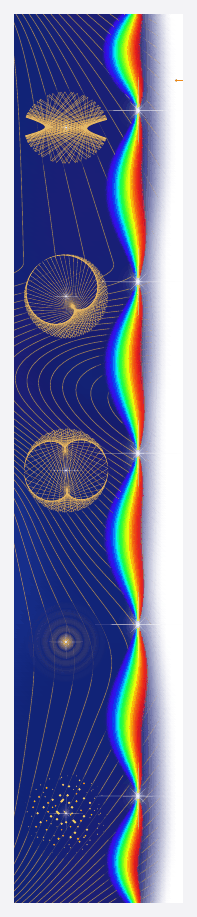
\includegraphics[width=\linewidth]{caustics.png}\end{minipage}\hfill
\begin{minipage}[c]{.76\linewidth}
\begin{itemize}
\item \opt{ellipse}. A ray inside an elliptical mirror. Orbits that nearly close, and so read as symbols, are rejected.
\item \opt{cardioid}. The caustic of a cup lit from a point on its rim, the shape at the bottom of a coffee mug.
\item \opt{nephroid}. The caustic of a cup in parallel light.
\item \opt{rings}. Diffraction by a round aperture, $(2J_1(x)/x)^2$ out to the fifth dark ring. The outer rings are lifted in brightness, or they would not show.
\item \opt{speckle}. A sum of waves with random directions and phases, as gold dust at the bright maxima.
\end{itemize}
\end{minipage}

\section{Printing}\label{paper}

\textbf{An office printer.} In the dark mode the margins cover about a quarter of the sheet, and an office printer does not print to the edge. For paper there is \opt{mode=paper}: the same construction on a light ground, a dark beam in place of the white one, and the spectrum appearing where it does in the night mode.

\fig[.84]{paper.png}{The same document with \opt{mode=paper}.}

In the gallery's example the mean darkness of a page falls from 27~\% to 7~\%. This is a rough measure taken from a rendering, not the ink a given printer uses. The mode has not been tried on a real printer yet.

\textbf{A print shop.} The option \opt{color=cmyk} draws everything in DeviceCMYK, and \opt{bleed=3} adds 3~mm on every side of the sheet and writes TrimBox and BleedBox. The art and the cover run past the trim line.
\begin{code}
\usepackage[cmyk]{xcolor}
\usepackage[color=cmyk,bleed=3]{limen}
\end{code}
The colour is converted by the plain formula without an ICC profile, and the saturated colours of the spectrum get noticeably duller in CMYK. The package makes no crop marks and no PDF/X. So ask the print shop for a proof before a run.

\textbf{A test sheet.} Before printing much, print one sheet of \opt{doc/limen-print-test.pdf}, also made by \opt{make print-test}. It has the stages of the beam at their real size, one fan in RGB and in CMYK, the dark fields of all palettes, lines from 0.2 to 1~pt, smooth ramps and text beside the edge of the field. Everything stays 10~mm from the edge, so the sheet fits an ordinary printer too. Print at 100~\%.

\section{The cover}

\cs{limencover\{title\}\{subtitle\}\{details\}} takes a whole page. The full spectrum is there at once, as a promise of how the document will end. With \opt{style=dark} the cover has only the white beam, and all of the colour stays for later. The cover does not count in the story but does take a page number: if needed, set \cs{setcounter\{page\}\{1\}} after it.

\section{Ornaments in the text}

The divider \cs{limenrule} suits a change of subject within a section:
\limenrule
The glint \limenspark{} stands in a line like a letter. The strip \limenspectrum[3cm] is handy in captions and legends. They are always drawn for a light page, in both modes.

\section{Slides}

The package detects the \opt{beamer} class by itself. The margin becomes a narrow column on the left, the overlays of one frame get one and the same picture, and the story counts frames, not PDF pages.

\begin{code}
\documentclass[aspectratio=169]{beamer}
\usepackage{limen}
\begin{document}
\begin{frame}[plain]\limencover{Title}{Subtitle}{Details}\end{frame}
\begin{frame}{Below the threshold} ... \end{frame}
\begin{frame}{The turn}\limenthreshold ... \end{frame}
\end{document}
\end{code}

\fig{slides.png}{The cover, a frame below the threshold and a frame above it.}

Set the width of the column on slides with a package option, \opt{column=2.2}, not through \cs{limensetup}: the text margin depends on it.

\section{Without LaTeX: SVG, Typst, the browser}

The drawing is separate from TeX, so the same file \opt{limen-art.lua} works without it.

\textbf{SVG.} One command draws one page. Any Lua 5.3 or later will do, such as \opt{texlua} from LuaTeX. Paths stay vector; the field and the beam become a PNG inside the file, because SVG has no colour meshes.
\begin{code}
texlua limen-svg.lua --page 3 --pages 8 --palette ruby > page-3.svg
texlua limen-svg.lua --help
\end{code}

\textbf{Typst.} The file \opt{typst/limen.typ} leaves marks at the headings, and \opt{typst/build.py} reads them, draws an SVG for each page and compiles the document with these as page backgrounds. Pages that have not changed are not drawn again.
\begin{code}
#import "limen.typ": limen, limen-threshold, limen-caustic
#show: limen

python3 typst/build.py report.typ --palette ultramarine
\end{code}
Typst sets its own text over the art. Initials, covers and ornaments in the text are not there yet.

\textbf{The browser.} The page \opt{web/index.html} tries out palette, threshold, beam and caustics on an eight-page sample and shows the result at once. Next to it are ready lines for LaTeX, Typst and the command line, and the address keeps the settings, so a result can be shared as a link. Lua runs there through Fengari, about 20 times slower than in LuaTeX, so the display is simplified: meshes are coarser than in a finished PDF. The button that copies an SVG draws the page at full quality. The paths come out the same, byte for byte. No server is needed: the page opens from a folder.

\section{Recipes}\label{recipes}

\textbf{A wide table in the middle.} The art follows the layout of each page, so changing the margins is enough:
\begin{code}
\clearpage\newgeometry{left=32mm,right=12mm}
... the table ...
\clearpage\restoregeometry
\end{code}
If the column has become too narrow, add \cs{limenpause} on that page.

\textbf{Appendices and references outside the story.} Put \cs{limenend} before them. The story ends there, and the following pages stay at the full stage.

\textbf{Your own headings.} Stars come by themselves in the headings of the standard classes, KOMA-Script, memoir and tagged documents. The package \opt{titlesec} replaces the heading code, so add the star to the format:
\begin{code}
\titleformat{\section}{\bfseries}{\thesection}{1em}{\limenstar}
\end{code}

\textbf{Two-sided printing.} With the class option \opt{twoside} and a wide outer margin, the art moves to the outer margin by itself and is reflected.

\textbf{Tinted paper.} The package must know the colour too, or the edge of the field fades to white:
\begin{code}
\usepackage[paper=FBF6EA]{limen}
\pagecolor[HTML]{FBF6EA}
\end{code}

\textbf{A tagged PDF.} Turn tagging on through \cs{DocumentMetadata}, and the package marks all of its art as an Artifact, so that screen readers pass over it. This needs LaTeX from 2024 or later.
\begin{code}
\DocumentMetadata{lang=en,tagging=on}
\documentclass{article}
\end{code}

\textbf{A different picture with the same story.} Change \opt{seed}. One file with one seed always gives one picture.

\textbf{Fast editing.} While working on the text, use the option \opt{draft}. The page breaks stay the same.

\textbf{The error cannot find file ''.} The font cache keeps the path by which a font was first loaded. If that path was relative, and another document takes a copy of the same file, with the same size and time, from another folder, LuaLaTeX stops with this error. It comes from the font loader and happens without limen too. An absolute \opt{Path} in \cs{setmainfont} helps, and so does deleting that font's file from the cache folder \opt{luatex-cache/generic/fonts/otl}. In a document with an initial, the package warns about this in the log beforehand.

\section{How it works}

\begin{itemize}
\item \textbf{One form per page.} All the art of a page goes into one PDF object (a Form XObject) with resources of its own. So the package does not depend on what other packages do with the page's resources.
\item \textbf{A transparency group of its own.} The page says which colour space to blend translucent lines and glows in, so that the viewer does not choose.
\item \textbf{Meshes, not stacks of contours.} Colour is painted with interpolating meshes (PDF shading type 5), smooth at any zoom.
\item \textbf{No blend modes.} Light is added up in Lua, and opaque colours go into the PDF. A Screen-blended mesh turned white in Poppler, which blends each triangle on its own.
\item \textbf{A computed spectrum.} The beam is a sum of Gaussian strands, one per wavelength, with conserved energy. So a narrow beam really adds up to white, and a wide one really separates into pure colours.
\item \textbf{Computed caustics.} Ray tracing, the geometry of envelopes and the diffraction formula.
\item \textbf{A measured ending.} On the closing page the real height of the content is taken from the finished page box, so floats and footnotes count, and the night field does not cover them.
\item \textbf{No dependence on the order of Lua tables.} Lines are walked in sorted order, and the random numbers do not depend on the width of integers, so the browser and LuaTeX compute the same thing.
\end{itemize}

One convention remains, and it matters: a real Nd:YAG beam is monochromatic and invisible (1064~nm). The rainbow is an image; the nearest physics is a supercontinuum. The scale of the lines and the bends of the beam are decorative.

The idea of drawing margins in Lua and the code that finds marks in the finished page come from the florilegium package by Kevin Raymond (MIT). The art, the story and the output are new, and florilegium is not needed.

\section{What has been checked and what has not}\label{checked}

\noindent\begin{tabularx}{\linewidth}{@{}P{26mm}L@{}}
\toprule
\thead{Checked} & \thead{With}\\\midrule
Building & A clean TeX Live 2026 (TinyTeX, LuaHBTeX 1.24.0, LaTeX 2026-06-01) and TeX Live 2023 (Debian, LuaHBTeX 1.17.0, LaTeX 2023-11-01, some packages added by hand)\\
Systems & Every push to GitHub is built on the current TeX Live: on Linux and macOS with all the checks, on Windows compilation and warnings only, because Poppler is not there\\
Classes & article, report, book, scrartcl, memoir, beamer\\
Layouts & A4, A5, Letter, landscape, two columns, two-sided, a narrow margin, a change of margins mid-document, tinted paper\\
Content & Russian (babel), fancyhdr, titlesec, hyperref, TikZ, floats and footnotes on the closing page, \cs{DocumentMetadata} tagging (2026 only)\\
Viewing & Poppler 24.02, PDFium 158 (the engine of Chrome), pdf.js 3.2: pages are compared automatically, see \opt{tools/crosscheck.py}. Adobe Acrobat on Windows: the cover, a page with figures and the last page looked over by hand\\
Without LaTeX & Typst 0.15.1. SVG compared with the PDF (\opt{tools/svgcheck.py}, up to 0.6~\% difference). The browser page tested in Chromium\\
Tests & 31 documents through \opt{make test}: the text with and without art is the same word for word, stars reach every heading, a repeated build gives the same pixels, CMYK and page boxes are there, warnings are only the expected ones\\
\bottomrule
\end{tabularx}

\medskip
\textbf{Not checked:} Preview on macOS, Ghostscript, MuPDF, real printing on a printer or at a print shop, MiKTeX, PDF/A and PDF/X. Tags have only been checked in the file's contents: no document has gone through the PAC or veraPDF validators.

\textbf{Speed and size.} Building takes about half a second per page, and a file grows by about 120~KB per page. Viewers based on Poppler (Evince, Okular) take 1--4~s to show a page, because Poppler cuts meshes into small pieces. PDFium and pdf.js take 0.02 to 0.3~s. When the zoom changes often, Acrobat redraws a page with a delay, and figures can vanish for that time.

\textbf{Known limits.}
\begin{itemize}
\item Text should stay out of the left margin: the art lies under it, and legibility there is not guaranteed.
\item With two columns, the last page gets no field below the text, only a small fan.
\item Automatic stars do not work with every kind of heading code. If they are missing, use \cs{limenstar}.
\item Starred headings (\cs{subsection*}) count as first-level and get a large star.
\end{itemize}

\section{What is left}

\textbf{Only a person can do this.}
\begin{itemize}
\item Open the files in Preview on a Mac, and print \opt{mode=paper} on an office printer. This is the largest remaining risk.
\item Put a name in \opt{LICENSE} and \opt{build.lua}, check the package name on CTAN and submit the archive that \opt{l3build ctan} makes.
\end{itemize}

\textbf{Tried and rejected.} Parametric meshes did not speed up Poppler. In a trial build Poppler became only slightly faster (1.3--1.7~s against 1.3--2.1~s per page), the file grew 3--4 times, and pdf.js slowed down dozens of times (10--12~s against 0.1--0.2~s). So plain meshes stayed.

\textbf{What could come next.}
\begin{itemize}
\item An ICC profile and PDF/X for print shops, in place of the plain CMYK formula.
\item Running the tags through validators, and a text description of the art for screen readers.
\item Initials, covers and ornaments in the Typst version.
\item Crop marks.
\end{itemize}

\bigskip
{\small\color{muted}MIT License, see \opt{LICENSE}. Fonts of this guide: Lora and Inter (SIL OFL). Hyphenation patterns: hyph-utf8 (LPPL). Lua in the browser: Fengari (MIT).\par}
\end{document}
